% Intended LaTeX compiler: lualatex
\documentclass{mcreport}
% org-mc-latex-classes.el --------------------------
% Additional LaTeX headers from #+LATEX_HEADER lines
% ==============================================================
% BEGIN SETUPFILE: latex-listings.setup
%
% Copyright (C) 2008-2026 Fabrice Niessen. All rights reserved.
%
% Purpose: Listings configuration for source code typesetting
%          and syntax highlighting.
% Scope:   LaTeX exports using the listings package;
%          applies to Beamer and other document classes.
% ==============================================================

% Typeset source code listings.
\usepackage{listings}

% --------------------------------------------------------------
% Colors.
% --------------------------------------------------------------
\usepackage{xcolor}
\definecolor{mc@lstidentifier}{HTML}{000000} % Black.
\definecolor{mc@lstcomment}{HTML}{008200}    % Green.
\definecolor{mc@lststring}{HTML}{FF5500}     % Orange.
\definecolor{mc@lstkeyword}{HTML}{0000FF}    % Blue.
\definecolor{mc@lstbackground}{HTML}{FFFDE7} % Warm light yellow.
\definecolor{mc@lstframe}{HTML}{F0E6A0}      % Soft yellow border.

\definecolor{mc@lstgitcmd}{HTML}{0000FF}      % Blue: git, cd, ls, ...
\definecolor{mc@lstgitsubcmd}{HTML}{008080}   % Teal: commit, log, merge, ...
\definecolor{mc@lstgitopt}{HTML}{CC5500}      % Dark orange: graph, oneline, cached, ...
\definecolor{mc@lstgitref}{HTML}{008200}      % Green: HEAD, origin/main, ...
\definecolor{mc@lstgitshortopt}{HTML}{AA0000} % Dark red: a, p, v, m, am, ...
\definecolor{mc@lstgboost}{HTML}{9900CC}      % Purple: GitBoost aliases.

% Colors for diff listings.
\definecolor{mc@diffstart}{HTML}{666666}   % Gray.
\definecolor{mc@diffadded}{HTML}{008200}   % Green.
\definecolor{mc@diffremoved}{HTML}{CC0000} % Red.

\definecolor{TeXbackgroundcolor}{HTML}{F1F9EF} % Very light green.
\definecolor{TeXrulecolor}{HTML}{D4E8E3}       % Pale green.

\definecolor{mc@examplebackground}{HTML}{EAF7EA} % Very light green.
\definecolor{mc@exampleframe}{HTML}{A8D5A8}      % Light green.

% --------------------------------------------------------------
% Languages.
% --------------------------------------------------------------
% Diff language for listings.
\lstdefinelanguage{diff}{%
morecomment=[f][\color{mc@diffstart}]{@@},% Hunk headers.
morecomment=[f][\color{mc@diffremoved}]-,% Removed lines.
morecomment=[f][\color{mc@diffadded}]+,% Added lines.
morecomment=[f][\color{mc@diffstart}]{---},% File headers (old).
morecomment=[f][\color{mc@diffstart}]{+++},% File headers (new).
}

% Plain text language for listings.
\lstdefinelanguage{text}{}

% Archibus log language for listings.
\lstdefinelanguage{ablog}{}

\lstdefinelanguage{conf}{
morecomment=[l]{\#},
morecomment=[l]{;},
morestring=[b]",
morestring=[b]',
sensitive=true
}

\lstdefinelanguage{org}{%
morekeywords={:exports, :noweb, :results, :session, :var},
sensitive=false,
morestring=[b]",
morecomment=[l]{\#},
}

% Shell commands with Git-aware highlighting.
\lstdefinelanguage{shell}{
% Generic shell commands and local command aliases.
morekeywords={
alias,apt,cat,cd,cp,echo,export,g,git,grep,
ls,mkdir,mv,pwd,rm,smerge,sudo,touch,wget
},
% Git subcommands and common Unix commands used in Git examples.
morekeywords=[2]{
add,apply,bad,bisect,blame,branch,checkout,cherry-pick,
clean,clone,commit,config,diff,difftool,fetch,good,head,
init,install,log,ls-files,merge,mergetool,pop,pull,push,
rebase,reflog,remote,reset,restore,revert,run,show,start,
stash,status,switch,tag,tail,xargs,zip
},
% Git long options without their leading dashes.
morekeywords=[3]{
abort,abbrev-commit,all,amend,autostash,cached,color-words,
continue,decorate,follow,force-with-lease,global,graph,
hard,keep,list,mixed,name-only,oneline,pretty,prune,rebase,
soft,sort,source,staged,stat,tags,track,word-diff-regex,
worktree
},
% Common Git references, remotes and branch names.
morekeywords=[4]{
FETCH_HEAD,HEAD,MERGE_HEAD,ORIG_HEAD,main,master,origin,
origin/main,origin/master
},
% Common short options without their leading dash.
morekeywords=[5]{
I,a,am,av,b,d,i,l,m,p,s,v,vv
},
% GitBoost aliases.
morekeywords=[6]{
% A
ack,
aliases,
all-repos,
amend-message,
amend-reuse,
% B
br,
branches,
branches-containing,
% C
changed-files,
co,
common-ancestor,
commit-interactive,
create-branch,
current-branch,
% D
delete-gone-branches,
delete-remote-branch,
df,
dfc,
dt,
dtc,
% F
file-history,
file-history-all-branches,
file-last-commit-all-local-branches,
find-commit-diffs-all-branches,
find-commit-messages-all,
find-commit-messages-any,
% G
gno,
grep-aliases,
grep-all-commits,
grep-all-local-branches,
grep-all-tracked-files,
grep-current-branch,
% I
ignore,
in,
incoming,
init-repository,
% L
lg-all-branches,
ll,
lll,
local-commit,
log-unified-diff,
ls,
% M
merge-test,
mindf,
mindfc,
minshow,
missing,
% N
no-ff,
% O
out,
outgoing,
% P
publish-branch,
pull-autostash,
% R
r,
record,
recommit,
related-files,
release-tag,
releases,
rename-branch,
rename-local-branch,
reword,
% S
search-for-code,
squash,
st,
stash-all,
stash-only-untracked,
% U
unadd,
uncommit,
uncommit-unadd,
uncommit-unstage,
unmodify,
unstage,
upstream-commit,
% W
wdf,
wdfc,
whoami,
wshow,
wwflu
},
keywordstyle=[1]\color{mc@lstgitcmd}\bfseries,
keywordstyle=[2]\color{mc@lstgitcmd}\bfseries,
keywordstyle=[3]\color{mc@lstgitopt},
keywordstyle=[4]\color{mc@lstgitref}\bfseries,
keywordstyle=[5]\color{mc@lstgitshortopt}\bfseries,
keywordstyle=[6]\color{mc@lstgboost}\bfseries,
%
% Treat lines starting with '#' as shell comments.
morecomment=[l]{\#},
%
% Treat '.' and '/' as part of identifiers so compound Git names
% such as feature/login and path-like references are highlighted
% as single keywords.
%
% The '-' character is intentionally excluded. Including it in
% alsoletter would cause options beginning with '-' (for example
% -a, --all, --graph or --force-with-lease) to be parsed as part
% of larger identifiers and prevent correct option highlighting.
alsoletter={./},
sensitive=true,
}

% --------------------------------------------------------------
% Styles.
% --------------------------------------------------------------
\lstdefinestyle{TeX}{
backgroundcolor=\color{TeXbackgroundcolor},
rulecolor=\color{TeXrulecolor}
}

\lstdefinestyle{example}{
language=shell, % text
backgroundcolor={},
}

% --------------------------------------------------------------
% Accessibility.
% Hide line numbers from copy/paste operations in PDF output.
% --------------------------------------------------------------
\usepackage{accsupp}

\newcommand{\emptyaccsupp}[1]{%
\BeginAccSupp{ActualText={}}#1\EndAccSupp{}%
}

\definecolor{mc@lstlinenumber}{gray}{0.75}

\newcommand{\lstnumberstyle}{%
\color{mc@lstlinenumber}%
\tiny\ttfamily\emptyaccsupp
}

% --------------------------------------------------------------
% Global listings defaults.
% --------------------------------------------------------------
\lstset{%
lineskip=-0.1em,
%
basicstyle=\ttfamily\scriptsize, % Font used for code.
identifierstyle=\color{mc@lstidentifier},
commentstyle=\color{mc@lstcomment}\itshape,
stringstyle=\color{mc@lststring},
keywordstyle=\color{mc@lstkeyword},
%
upquote,
tabsize=4, % Set the default tab size to 4 spaces.
showtabs=false, % Show tabs within strings using underscores.
%  tab=$\to$,
showspaces=false, % Show spaces using underscores.
showstringspaces=false, % Underline spaces within strings.
%
numbers=left, % Position of line numbers.
numberstyle=\lstnumberstyle, % Line number style.
%
captionpos=b, % Place captions below listings.
%
xleftmargin=0.4em, % Text to the right.
xrightmargin=0.4em, % Text to the left.
breaklines=true, % Visually wrap long listing lines when possible.
breakatwhitespace=true, % Prefer whitespace as a visual wrap point.
%
frame=single, % Draw a frame around listings.
framexleftmargin=0pt, % Left frame margin.
framexrightmargin=0pt, % Right frame margin.
backgroundcolor=\color{mc@lstbackground}, % Background color.
rulecolor=\color{mc@lstframe}, % Frame color.
%
columns=flexible, % Use flexible character widths instead of fixed columns.
keepspaces=true, % Preserve consecutive spaces and indentation.
%
% mathescape, % Allow escaping to (La)TeX mode within $..$.
%
% Display placeholders between ⟨ and ⟩, in italic and in a specific color.
moredelim={[s][\itshape\color{brown}]{⟨}{⟩}},
}

% --------------------------------------------------------------
% Unicode support for listings.
% --------------------------------------------------------------
% Extend listings' internal character table to recognize Unicode
% code points above 255. This allows characters such as ⟨, ⟩ and
% horizontal ellipsis to be processed correctly when using
% modern Unicode engines (LuaLaTeX and XeLaTeX).
\makeatletter
\lst@InputCatcodes
\def\lst@DefEC{%
\lst@CCECUse \lst@ProcessLetter
^^80^^81^^82^^83^^84^^85^^86^^87^^88^^89^^8a^^8b^^8c^^8d^^8e^^8f%
^^90^^91^^92^^93^^94^^95^^96^^97^^98^^99^^9a^^9b^^9c^^9d^^9e^^9f%
^^a0^^a1^^a2^^a3^^a4^^a5^^a6^^a7^^a8^^a9^^aa^^ab^^ac^^ad^^ae^^af%
^^b0^^b1^^b2^^b3^^b4^^b5^^b6^^b7^^b8^^b9^^ba^^bb^^bc^^bd^^be^^bf%
^^c0^^c1^^c2^^c3^^c4^^c5^^c6^^c7^^c8^^c9^^ca^^cb^^cc^^cd^^ce^^cf%
^^d0^^d1^^d2^^d3^^d4^^d5^^d6^^d7^^d8^^d9^^da^^db^^dc^^dd^^de^^df%
^^e0^^e1^^e2^^e3^^e4^^e5^^e6^^e7^^e8^^e9^^ea^^eb^^ec^^ed^^ee^^ef%
^^f0^^f1^^f2^^f3^^f4^^f5^^f6^^f7^^f8^^f9^^fa^^fb^^fc^^fd^^fe^^ff%
% Additional Unicode characters.
^^^^20ac^^^^0153^^^^0152% €, œ, Œ
^^^^2194% Left-right arrow.
^^^^27e8% Left angle bracket.
^^^^27e9% Right angle bracket.
^^^^2026% Horizontal ellipsis.
^^00}
\lst@RestoreCatcodes
\makeatother

% --------------------------------------------------------------
% Inline command boxes.
% Used by Org macros ikbd and kbd.
% Requires: listings and tcolorbox.
% --------------------------------------------------------------
\usepackage{tcolorbox}

\tcbset{
commandboxstyle/.style={
on line,
nobeforeafter,
boxsep=1pt,
left=2pt,
right=2pt,
top=1pt,
bottom=1pt,
colback=black!10
}
}

\NewTotalTCBox{\commandbox}{ s O{} m }
{commandboxstyle, boxrule=0.3pt, colframe=black!45}
{%
\IfBooleanT{#1}{\textcolor{red}{\ttfamily\bfseries \$ }}%
\lstinline[language=shell,#2]§#3§%
}

\NewTotalTCBox{\lightcommandbox}{ s O{} m }
{commandboxstyle, boxrule=0pt, colframe=black!10}
{%
\IfBooleanT{#1}{\textcolor{red}{\ttfamily\bfseries \$ }}%
\lstinline[language=shell,#2]§#3§%
}

% --------------------------------------------------------------
% Terminal sessions.
% Requires: listings, tcolorbox and accsupp.
% --------------------------------------------------------------
% Style used for shell sessions displayed in a terminal-like box.
\lstdefinestyle{terminal}{
language=shell, % text
backgroundcolor=,
frame=none,
numbers=none,
basicstyle=\scriptsize\ttfamily,
moredelim={[s][\itshape\color{brown}]{⟨}{⟩}},
}

% Prompt displayed at the beginning of each command line.
\newcommand{\terminalprompt}{%
\bfseries%
% \textcolor{cyan}{alice\textcolor{gray}{@}ubuntu}%
% \textcolor{gray}{:}%
% \textcolor{lime!50!black}{\~{}}%
\textcolor{red!50}{\$}%
}

\tcbuselibrary{listings}

% Terminal environment used by Org's #+begin_terminal blocks.
\lstnewenvironment{terminal}[1][]
{%
\lstset{%
language=shell,
style=terminal,
basicstyle=\ttfamily\scriptsize,
moredelim={[l][\color{black}]{\#\#}},
escapeinside=£\ ,
escapebegin=\BeginAccSupp{ActualText={}}\pause{}\terminalprompt\EndAccSupp{},
escapeend=\BeginAccSupp{ActualText={}}\ \EndAccSupp{},
backgroundcolor=\color{violet!10!white},
rulecolor=\color{gray!65!black},
#1
}%
}
{}

% ==============================================================
% END SETUPFILE: latex-listings.setup
% ==============================================================
% ==============================================================
% BEGIN SETUPFILE: latex-admonitions.setup
% Purpose: Read the Docs-style admonition and task boxes
% Scope: LaTeX exports using standard classes and Beamer
% ==============================================================
% Read the Docs-style admonition and callout boxes.
\usepackage{boostboxes}
% ==============================================================
% END SETUPFILE: latex-admonitions.setup
% ==============================================================
\usepackage{amssymb} % Required for examples using \checkmark, \square, etc.

% End of org-mc-latex-classes.el -------------------
\author{Fabrice Niessen}
\date{\today}
\title{Comprehensive Org mode syntax and features reference}
\hypersetup{
 pdfauthor={Fabrice Niessen},
 pdftitle={Comprehensive Org mode syntax and features reference},
 pdfkeywords={Org mode, syntax, markup, documentation},
 pdfsubject={Examples of Org mode markup, export features, Babel, tables, links, drawers, and advanced document elements.},
 pdfcreator={Emacs 30.2 (Org mode 9.7.11)}, 
 pdflang={English}}
\begin{document}

\maketitle
\setcounter{tocdepth}{2}
\tableofcontents

This document demonstrates a broad range of Org mode features. It serves as
a comprehensive reference for writing technical documentation, producing HTML
and PDF output, embedding source code, and testing CSS, \LaTeX{}, and export
behavior.

\textbf{Org mode} provides a simple \emph{plain-text} markup language for creating
well-structured documents. From a single source file, you can produce
high-quality HTML, \LaTeX{}, PDF, and many other output formats while maintaining
an efficient writing workflow.
\chapter{Basics}
\label{sec:orgbaff123}

This chapter introduces the fundamental building blocks of an Org document.
\section{Biggest heading}
\label{sec:org3339894}

Start a new chapter by creating a top-level heading.
\subsection{Bigger heading}
\label{sec:org11da43b}

Use section headings to organize related content.
\subsubsection{Big heading}
\label{sec:orgad94917}

Subsections help divide longer sections into manageable parts.
\subsubsection{Paragraphs and line breaks}
\label{sec:org88476f2}

A single newline does not create a new paragraph.
The following lines belong to the same paragraph.

But an empty line

demarcates a new paragraph.

To force a line break without beginning a new paragraph, end a line with
2 backslashes. \\
The next line will appear immediately below it.

To insert a horizontal rule, write at least 5 consecutive hyphens: this text
appears above the horizontal rule.

\noindent\rule{\textwidth}{0.5pt}
and this text appears below it.
\subsubsection{Numbered headings}
\label{sec:org74ae2a4}

You can automatically number headings up to a specified depth by setting the
appropriate export option.

\begin{lstlisting}[language=org,numbers=none]
#+OPTIONS: H:4
\end{lstlisting}
\subsection{Text width}
\label{sec:org0fe24ac}

The following paragraph is intentionally long to demonstrate line wrapping and
text formatting during export.

One morning, when Gregor Samsa woke from troubled dreams, he found himself
transformed in his bed into a horrible vermin. He lay on his armour-like back,
and if he lifted his head a little he could see his brown belly, slightly domed
and divided by arches into stiff sections. The bedding was hardly able to cover
it and seemed ready to slide off any moment. His many legs, pitifully thin
compared with the size of the rest of him, waved about helplessly as he looked.
\section{Lists}
\label{sec:org68e2f2e}

Org mode provides several types of lists that can be freely combined to organize
information clearly and consistently.
\subsection{Unordered lists}
\label{sec:org1b528f7}

Bulleted lists are useful for presenting related information without implying
a particular order.

They are commonly used to:

\begin{itemize}
\item organize information, and
\item present content
\begin{itemize}
\item hierarchically, and
\item easy to read.
\end{itemize}
\end{itemize}

You can begin list items with either a minus (\lstinline|-|) or a plus sign (\lstinline|+|).
\subsection{Ordered lists}
\label{sec:org11bd972}

Numbered lists express sequences or ordered procedures.

\begin{enumerate}
\item First item
\begin{enumerate}
\item First sub-item
\item Second sub-item
\end{enumerate}
\item Second item
\end{enumerate}

You can also specify explicit numbering when necessary:

\begin{enumerate}
\setcounter{enumi}{0}
\item First item
\setcounter{enumi}{1}
\item Second item
\setcounter{enumi}{4}
\item Continue with item 5
\end{enumerate}
\subsection{Definition lists}
\label{sec:orgae7629a}

Definition lists associate terms with descriptions.

\begin{description}
\item[{Definition list}] A list in which each item consists of a term followed by its definition.

\item[{Org mode}] A powerful plain-text authoring system built into Emacs.
\end{description}
\subsection{Checklists}
\label{sec:orga85222c}

Checkboxes make it easy to track progress.

\begin{itemize}
\item[{$\square$}] Incomplete task
\item[{$\boxminus$}] Task in progress
\begin{itemize}
\item[{$\boxtimes$}] First subtask
\item[{$\square$}] Second subtask
\end{itemize}
\item[{$\boxtimes$}] Completed task
\end{itemize}
\section{Additional features}
\label{sec:orgc02fb54}

\subsection{Including other Org files}
\label{sec:orge5ab6b4}

You can include the contents of another Org file during export. For example, the
following directive imports the referenced file while skipping its title:

\begin{lstlisting}[language=org,numbers=none]
#+INCLUDE: chapter1.org :lines "2-"
\end{lstlisting}

\begin{note}
File inclusion using the \lstinline|#+INCLUDE| keyword is supported \textbf{during export only}.
\end{note}
\subsection{Inline HTML}
\label{sec:org84942de}

Raw HTML can be embedded directly in an Org document. When exporting to HTML,
the markup is preserved exactly as written.

This text appears in a fixed-width font only in HTML.
Embedding raw HTML is particularly useful when you need functionality beyond Org
mode's built-in export options, such as custom markup, advanced styling, or
interactive content.

For example, you can define custom HTML containers that correspond to CSS
classes:

\begin{verbatim}
#+begin_info
*Info example* \\
Additional details appear here.
#+end_info
\end{verbatim}

You may also embed JavaScript, interactive visualizations (such as interactive
R plots), or other HTML elements when appropriate.

To include an existing HTML file verbatim during export:

\begin{lstlisting}[language=org,numbers=none]
#+INCLUDE: file.html html
\end{lstlisting}

Changes should always be made to the original Org source rather than the
exported HTML output!
\subsection{Inline \LaTeX{}}
\label{sec:orgb5804a0}

Raw \LaTeX{} may also be embedded directly in an Org document.

\begin{verbatim}
This text is displayed in a fixed-width font only in \LaTeX{}.
\end{verbatim}
\subsection{Centered text}
\label{sec:orgaffb413}

Use a \lstinline|center| block to center its contents.

\begin{center}
This text is centered.
\end{center}
\section{Code blocks}
\label{sec:org540ceb3}

Source code blocks are one of Org mode's most powerful features. They support
syntax highlighting, executable code through Org Babel, export to multiple
formats, and \textbf{reproducible research} workflows.
\subsection{Diff}
\label{sec:orgee031b4}

Unified diffs are useful for illustrating changes between two versions of
a file.

\begin{lstlisting}[language=diff,numbers=none]
diff --git a/config.org b/config.org
index 1a2b3c4..5d6e7f8 100644
--- a/config.org
+++ b/config.org
@@ -1,6 +1,7 @@
 #+TITLE: Example document
 #+AUTHOR: Alice
+#+LANGUAGE: en

-* Introduction
+* Getting started

-This is the original paragraph.
+This is the updated paragraph with clearer wording.
\end{lstlisting}
\subsection{\LaTeX{}}
\label{sec:org844694f}

\begin{lstlisting}[language={[LaTeX]TeX},numbers=none]
\documentclass[a4paper,11pt]{article}

\usepackage[T1]{fontenc}
\usepackage{amsmath,amssymb}
\usepackage{graphicx}
\usepackage{xcolor}
\usepackage{hyperref}

\title{Syntax Highlighting Demo}
\author{Fabrice Niessen}
\date{\today}

\begin{document}

\maketitle

\section{Introduction}

This is a simple demonstration of \LaTeX{} syntax.

Inline math: \(e^{i\pi} + 1 = 0\).

Displayed equation:

\[
\int_0^\infty e^{-x^2}\,dx = \frac{\sqrt{\pi}}{2}.
\]

A numbered equation:

\begin{equation}
\nabla \cdot \mathbf{E} = \frac{\rho}{\varepsilon_0}.
\end{equation}

\subsection{Lists}

\begin{itemize}
  \item First item
  \item Second item with \textbf{bold} and \emph{emphasis}
  \item A colored word: \textcolor{blue}{blue}
\end{itemize}

\subsection{Table}

\begin{tabular}{lcr}
\hline
Name  & Value & Unit \\
\hline
Speed &    42 & m/s  \\
Mass  &   5.3 & kg   \\
\hline
\end{tabular}

\subsection{Figure}

\begin{figure}[h]
  \centering
  \includegraphics[width=0.4\textwidth]{example-image}
  \caption{An example image.}
\end{figure}

A hyperlink: \url{https://www.latex-project.org}

\end{document}
\end{lstlisting}
\subsection{Line numbers}
\label{sec:org216e817}

Both \lstinline|example| and \lstinline|src| blocks support optional line numbering. Add the \lstinline|-n|
switch to the \lstinline|#+begin| line to display line numbers.

\begin{lstlisting}[language=Lisp,firstnumber=1,numbers=left]
(defun org-xor (a b)
  "Exclusive or."
\end{lstlisting}

To continue numbering from a previous numbered block, use the \lstinline|+n| switch.

\begin{lstlisting}[language=Lisp,firstnumber=3,numbers=left]
  (if a (not b) b))
\end{lstlisting}

Literal example blocks can also define labels such as \lstinline|(ref:name)|. These labels
become reference targets that may be linked elsewhere in the document, using
special hyperlinks like \lstinline|[[(name)]]| (i.e., with the reference name enclosed in
single parenthesis).

(In HTML, hovering the mouse over such a link will remote-highlight the
corresponding code line, which is kind of cool.)

Use the \lstinline|-r| switch to suppress labels in the exported source while still
allowing references.

With the \lstinline|-n| switch, links to these references will be labeled by the line
numbers from the code listing, otherwise links will use the labels with no
parentheses.

\begin{lstlisting}[language=Lisp,firstnumber=1,numbers=left]
  (save-excursion                  ;
    (goto-char (point-min)))       ;
\end{lstlisting}

In line 1, the current cursor position is saved. Line (jump) moves directly
to \lstinline|point-min|.
\subsection{Program output}
\label{sec:org24223e1}

One of Org mode's most powerful features is the ability to \textbf{execute} code and
insert its output directly into the document. This enables \emph{reproducible
research}.
\subsubsection{Text output}
\label{sec:org861be38}

A simple example:

\begin{lstlisting}[language=shell,numbers=none]
date +"%Y-%m-%d"
\end{lstlisting}

\phantomsection
\label{orga4f7d1c}
\begin{verbatim}
2026-08-12
\end{verbatim}


Longer command output may also be inserted into the document.

\begin{lstlisting}[language=shell,label=lst:org1d9a741,numbers=none]
# Output all styles, but the default one (if any).
ls ../src/ | grep -v "default"
\end{lstlisting}

\phantomsection
\label{orgd3606d4}
\begin{verbatim}
bigblow
readtheorg
vendor
\end{verbatim}
\subsubsection{Graphics}
\label{sec:orgbaf6dcb}

Data to be plotted:

\begin{table}[!htbp]
\label{tab:org359502a}
\centering
\begin{tabular}{rr}
Month & Degrees\\
\hline
1 & 3.8\\
2 & 4.1\\
3 & 6.3\\
4 & 9.0\\
5 & 11.9\\
6 & 15.1\\
7 & 17.1\\
8 & 17.4\\
9 & 15.7\\
10 & 11.8\\
11 & 7.7\\
12 & 4.8\\
\end{tabular}
\end{table}

The following R code generates a plot from the table above.

\begin{lstlisting}[language=r,label=lst:org91657a5,numbers=none]
plot(data, type = "b", bty = "l", col = c("#ABD249"), lwd = 4, las = 1)
grid(nx = NULL, ny = NULL, col = c("#E8E8E8"), lwd = 1)
legend("bottom", legend = c("Degrees"), col = c("#ABD249"), pch = c(19))
\end{lstlisting}

Generated figure:

\begin{center}
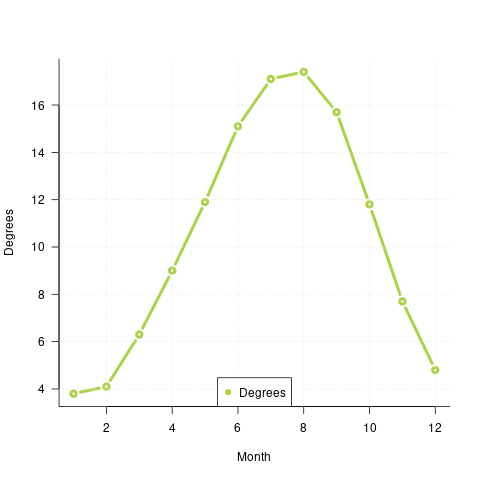
\includegraphics[width=.75\linewidth]{../images/Rplot.png}
\label{org22797de}
\end{center}
\subsubsection{R code example}
\label{sec:orgc6d6df7}

\begin{lstlisting}[language=r,numbers=none]
library(ggplot2)
summary(cars)
\end{lstlisting}

Example plot:

\begin{lstlisting}[language=r,numbers=none]
library(ggplot2)
qplot(speed, dist, data = cars) + geom_smooth()
\end{lstlisting}
\section{Inline code}
\label{sec:org842cb45}

Inline source blocks can be evaluated directly within normal text.

For example, 1 + 1 evaluates to .
\section{Text formatting}
\label{sec:org12a3dfa}

\subsection{Emphasis}
\label{sec:orgf8bf6b1}

Org mode supports several forms of inline emphasis.

Examples include:

\begin{itemize}
\item \emph{italic} for emphasis, book titles, or introducing new terms.
\item \textbf{bold} for strong emphasis or important information.
\item \textbf{\emph{bold italic}} for very strong emphasis.
\item \uline{underlined} for text that should appear underlined, such as headings or terms
that require visual emphasis.
\item \lstinline|inline code| for program code such as \lstinline|printf("hi")|, commands such as
\lstinline|git status|, variable names, function names such as \lstinline|strlen()|, or language
keywords.
\item \verb|verbatim text| for exact strings such as \verb|YES|, command-line options such as
\verb|--force-with-lease|, filenames such as \verb|README.org|, or any text that should be
reproduced exactly.
\item \sout{deleted text} for text that has been removed, is obsolete, or should be
ignored.
\item superscripts such as m/s\textsuperscript{2}
\item subscripts such as H\textsubscript{2}O
\end{itemize}

\textbf{Markup recognition rules}

Formatting can be nested.

For example, \emph{italic text containing \uline{underlined text} within it.}

Inline markup must be surrounded by appropriate boundaries and cannot be
embedded within a word.

For example, foo*bold*bar is not recognized because the markup is embedded
within a word.

By default, emphasis markup cannot span more than \textbf{2 consecutive lines}. For
example, the following is not recognized as bold text:

\textbf{This
is not
bold}
\subsection{Quotations}
\label{sec:org88ddd8a}

Use a \lstinline|quote| block for quoted prose.

\begin{quote}
Let us change our traditional attitude to the construction of programs:
Instead of imagining that our main task is to instruct a computer what to do,
let us concentrate rather on explaining to human beings what we want a
computer to do.

The practitioner of literate programming can be regarded as an essayist, whose
main concern is with exposition and excellence of style. Such an author, with
thesaurus in hand, chooses the names of variables carefully and explains what
each variable means. He or she strives for a program that is comprehensible
because its concepts have been introduced in an order that is best for human
understanding, using a mixture of formal and informal methods that reinforce
each other.

--- Donald Knuth
\end{quote}

Short quotations are equally straightforward.

\begin{quote}
Everything should be made as simple as possible,
but not any simpler. -- Albert Einstein
\end{quote}

A \lstinline|verse| block preserves indentation and line breaks exactly as written.

\begin{verse}
Everything should be made as simple as possible,\\
but not any simpler. -- Albert Einstein\\
\end{verse}

Verse blocks are also useful for preserving the formatting of email
conversations.

\begin{verse}
>> This is an email containing nested quotations.\\
>> Each level of indentation is preserved.\\
>\\
> Replies remain visually distinct from the original message.

Bullet lists may also appear inside verse blocks:\\
- First item\\
- Second item

Numbered lists are equally valid:\\
1. First item\\
2. Second item

Maybe an equation here?

See \url{https://www.google.com/} for additional information\ldots{}\\
\end{verse}
\subsection{Spaces}
\label{sec:org96a1b3a}

Non-breaking spaces may be inserted using the Unicode character \lstinline|U+00A0| or an
appropriate Org entity, depending on your export requirements.
\section{Mathematical expressions}
\label{sec:org5b28ddf}

Org mode supports \LaTeX{} mathematics in both HTML (via MathJax) and \LaTeX{}/PDF
exports.

\begin{itemize}
\item For \textbf{inline mathematics}, use \lstinline|\(...\)|: \(x^2\) or \(1 < 2\).

Although \lstinline|$...$| is commonly used in \LaTeX{}, \lstinline|\(...\)| is preferred in Org
documents.

\item Display equations appear centered on their own line (the \emph{Euler theorem}):

\[
  \int_0^\infty e^{-x^2} dx = \frac{\sqrt{\pi}}{2}
  \]

Display math using \lstinline|\[...\]| is useful whenever an equation deserves \textbf{visual
emphasis}.

For example, the \emph{quadratic formula} may be written as:
\[ \frac{-b \pm \sqrt{b^2 - 4ac}}{2a} \]

\textbf{Double dollar signs (\lstinline|$$|) should not be used}.

\item For \textbf{numbered} equations, use the \lstinline|equation| environment. The \emph{sinus theorem} can
then be written as the equation:

\begin{equation}
  \label{eqn:sinalpha}
  \frac{\sin\alpha}{a}=\frac{\sin\beta}{b}
\end{equation}

\item Equation references are also supported.

See Equation \ref{eq:orge92f284}.

\begin{equation}
\label{eq:orge92f284}
  n_{i+1}= \frac{n_{i}(d-i)(e-1)}{(i+1)}
\end{equation}

Only captioned equations receive automatic numbering.

\item If numbering is not required, use \lstinline|equation*|, \lstinline|displaymath|, or the shorter
\lstinline|\[...\]| syntax.
\end{itemize}
\section{Special characters}
\label{sec:orga50d76a}

Org mode provides convenient entities for many commonly used symbols.
\subsection{Accented characters}
\label{sec:orgad9c428}

\`{A} \'{A}
\subsection{Punctuation}
\label{sec:orgcccd2a8}

Dash: -- ---

Inverted punctuation: !` ?`

Quotation marks: \guillemotleft{} \guillemotright{}

Other symbols: \P{} \textordfeminine{}
\subsection{Commercial symbols}
\label{sec:org1b4f088}

Copyright: \textcopyright{}

Registered trademark: \textregistered{}

Currency: \textcent{} \texteuro{} \textyen{} \pounds{}
\subsection{Greek letters}
\label{sec:orgb66d063}

The Greek letters \(\alpha\), \(\beta\), and \(\gamma\) are used to denote angles in mathematics.
\subsection{Mathematical symbols}
\label{sec:org083f80c}

Arithmetic: \textpm{} \textdiv{}

Arrows: \(\to\) \(\rightarrow\) \(\leftarrow\) \(\leftrightarrow\) \(\Rightarrow\) \(\Leftarrow\) \(\Leftrightarrow\)

Functions: \(\arccos\) \(\cos\)

Additional symbols: \textbullet{} \(\star\)
\subsection{Miscellaneous symbols}
\label{sec:org0963640}

Card suits: \(\clubsuit\) \(\spadesuit\)
\section{Comments}
\label{sec:orgee40b77}

Comments may be placed anywhere in an Org document.

Lines beginning with \lstinline|#| are ignored during export.
\section{Tables}
\label{sec:org5ee3b96}

Org mode makes it easy to create and maintain tables.

\begin{table}[!htbp]
\caption{Example table}
\centering
\begin{tabular}{lll}
Header 1 & Header 2 & Header 3\\
\hline
Top left & Top middle & \\
 &  & Right\\
Bottom left & Bottom middle & \\
\end{tabular}
\end{table}

Columns are aligned automatically.

\begin{itemize}
\item Numeric columns are right-aligned.
\item Text columns are left-aligned.
\end{itemize}

Alignment can also be specified explicitly.

\begin{table}[!htbp]
\caption{Table with explicit alignment}
\centering
\begin{tabular}{rcl}
1 & 2 & 3\\
right & center & left\\
xxxxxxxxxxxx & xxxxxxxxxxxx & xxxxxxxxxxxx\\
\end{tabular}
\end{table}

Placement may be controlled during \LaTeX{} export.

\begin{tabular}{rr}
a & b\\
\hline
1 & 2\\
\end{tabular}

This differs from the default centered table.

\begin{center}
\begin{tabular}{rr}
a & b\\
\hline
1 & 2\\
\end{tabular}
\end{center}
\subsection{Table alignment on the page}
\label{sec:orgb8c31b1}

Left-aligned table:

\noindent
\begin{tabular}{rrr}
a & b & c\\
\hline
1 & 2 & 3\\
4 & 5 & 6\\
\end{tabular}
\hfill

The \lstinline|noindent| just gets rid of the indentation of the first line of a paragraph
which in this case is the table, and the \lstinline|hfill| adds infinite stretch after the
table, so it pushes the table to the left.

Centered table:

\begin{center}
\begin{tabular}{rrr}
a & b & c\\
\hline
1 & 2 & 3\\
4 & 5 & 6\\
\end{tabular}
\end{center}

Right-aligned table:

\hfill
\begin{tabular}{rrr}
a & b & c\\
\hline
1 & 2 & 3\\
4 & 5 & 6\\
\end{tabular}

Here, the \lstinline|hfill| adds infinite stretch before the table, so it pushes the table
to the right.
\subsection{Long tables}
\label{sec:org7a289ba}

Long tables may span multiple pages when exporting to PDF. Depending on the
\LaTeX{} configuration, table headers can automatically be repeated at the top of
each page.

\begin{table}[!htbp]
\caption{Example of a long table}
\centering
\begin{tabular}{rlllll}
Row & Project & Owner & Status & Priority & Estimate\\
\hline
1 & Alpha & Alice & Done & High & 2 d\\
2 & Bravo & Bob & In Progress & Medium & 5 d\\
3 & Charlie & Carol & Planned & Low & 3 d\\
4 & Delta & David & Done & High & 1 d\\
5 & Echo & Emma & Planned & Medium & 4 d\\
6 & Foxtrot & Frank & Done & High & 2 d\\
7 & Golf & Grace & Planned & Low & 8 d\\
8 & Hotel & Henry & Done & Medium & 3 d\\
9 & India & Irene & In Progress & High & 6 d\\
10 & Juliet & John & Planned & Low & 7 d\\
11 & Kilo & Kate & Done & High & 2 d\\
12 & Lima & Luke & In Progress & Medium & 5 d\\
13 & Mike & Mary & Planned & Low & 3 d\\
14 & November & Neil & Done & High & 1 d\\
15 & Oscar & Olivia & Planned & Medium & 4 d\\
16 & Papa & Peter & Done & High & 2 d\\
17 & Quebec & Quinn & Planned & Low & 8 d\\
18 & Romeo & Rose & Done & Medium & 3 d\\
19 & Sierra & Steve & In Progress & High & 6 d\\
20 & Tango & Tina & Planned & Low & 7 d\\
21 & Uniform & Uma & Done & High & 2 d\\
22 & Victor & Victor & In Progress & Medium & 5 d\\
23 & Whiskey & Wendy & Planned & Low & 3 d\\
24 & Xray & Xavier & Done & High & 1 d\\
25 & Yankee & Yvonne & Planned & Medium & 4 d\\
26 & Zulu & Zach & Done & High & 2 d\\
27 & Alpha & Alice & Planned & Low & 8 d\\
28 & Bravo & Bob & Done & Medium & 3 d\\
29 & Charlie & Carol & In Progress & High & 6 d\\
30 & Delta & David & Planned & Low & 7 d\\
31 & Echo & Emma & Done & High & 2 d\\
32 & Foxtrot & Frank & In Progress & Medium & 5 d\\
33 & Golf & Grace & Planned & Low & 3 d\\
34 & Hotel & Henry & Done & High & 1 d\\
35 & India & Irene & Planned & Medium & 4 d\\
36 & Juliet & John & Done & High & 2 d\\
37 & Kilo & Kate & Planned & Low & 8 d\\
38 & Lima & Luke & Done & Medium & 3 d\\
39 & Mike & Mary & In Progress & High & 6 d\\
40 & November & Neil & Planned & Low & 7 d\\
41 & Oscar & Olivia & Done & High & 2 d\\
42 & Papa & Peter & In Progress & Medium & 5 d\\
43 & Quebec & Quinn & Planned & Low & 3 d\\
44 & Romeo & Rose & Done & High & 1 d\\
45 & Sierra & Steve & Planned & Medium & 4 d\\
46 & Tango & Tina & Done & High & 2 d\\
47 & Uniform & Uma & Planned & Low & 8 d\\
48 & Victor & Victor & Done & Medium & 3 d\\
49 & Whiskey & Wendy & In Progress & High & 6 d\\
50 & Xray & Xavier & Planned & Low & 7 d\\
51 & Yankee & Yvonne & Done & High & 2 d\\
52 & Zulu & Zach & In Progress & Medium & 5 d\\
53 & Alpha & Alice & Planned & Low & 3 d\\
54 & Bravo & Bob & Done & High & 1 d\\
55 & Charlie & Carol & Planned & Medium & 4 d\\
56 & Delta & David & Done & High & 2 d\\
57 & Echo & Emma & Planned & Low & 8 d\\
58 & Foxtrot & Frank & Done & Medium & 3 d\\
59 & Golf & Grace & In Progress & High & 6 d\\
60 & Hotel & Henry & Planned & Low & 7 d\\
\end{tabular}
\end{table}
\section{Images, video, and audio}
\label{sec:orgc339ff8}

\subsection{Images}
\label{sec:org8daf990}

Org mode supports several image formats.

\begin{center}
\begin{tabular}{lll}
Format & HTML & PDF\\
\hline
GIF & Yes & \\
JPEG & Yes & \\
PNG & Yes & \\
BMP & Browser dependent & \\
\end{tabular}
\end{center}

Example image:

\begin{figure}[!htbp]
\centering

\includegraphics[width=0.25\linewidth]{../images/org-mode-unicorn.png}
\caption{Org mode logo}
\end{figure}

You may also link directly to an image file.

\href{../images/org-mode-unicorn.png}{Org mode unicorn image}

Common HTML image attributes include:

\begin{itemize}
\item \lstinline|align|
\item \lstinline|border|
\item \lstinline|bordercolor|
\item \lstinline|hspace|
\item \lstinline|vspace|
\item \lstinline|width|
\item \lstinline|height|
\item \lstinline|title|
\item \lstinline|alt|
\end{itemize}

Multiple images can also be arranged side by side using appropriate export
options.
\subsection{Video}
\label{sec:org11ca0b7}

Video files are typically referenced through hyperlinks.

A common approach is to use a thumbnail image that links to the video.

\href{https://www.youtube.com/shorts/ev1d8wowPuM}{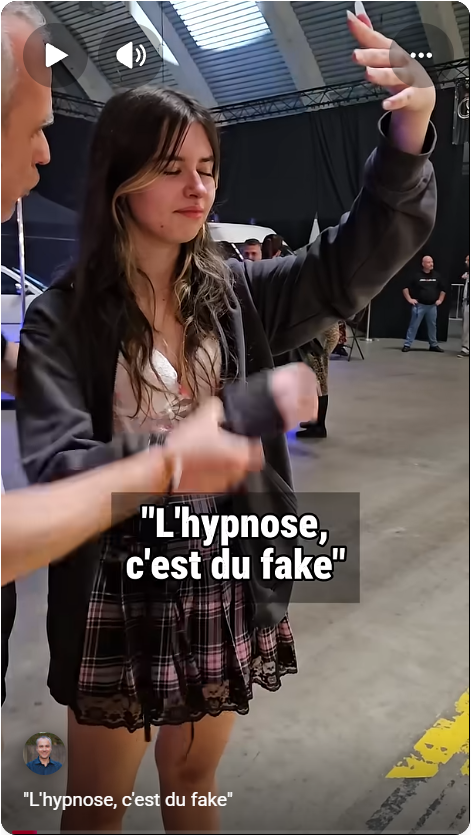
\includegraphics[width=.75\linewidth]{../images/l-hypnose-c-est-du-fake.png}}
\subsection{Audio}
\label{sec:orga62f7c7}

Audio resources may be linked using standard Org hyperlinks.
\section{Special text boxes}
\label{sec:org6b8360e}

Org mode supports several block types for emphasizing content.
\subsection{Inline tasks}
\label{sec:org8e6ca05}

Inline tasks can be used to record reminders or small tasks directly within a
document. They may include a TODO keyword, a priority, and tags.

An inline task with a description:

\begin{boostinlinetask}[TODO]{Write the introduction}
Draft the introductory section before the next review meeting.
\end{boostinlinetask}

A compact inline task without a description:

\boostcompacttask[WAIT]{{\setlength{\fboxsep}{1pt}\fbox{\#A}}\hspace{0.4em}Contact the customer}[phone]
\subsection{Example}
\label{sec:org667a12c}

Example blocks display literal text exactly as written.

Find entries containing an \textbf{exact phrase} by enclosing the phrase in quotation
marks:

\begin{verbatim}
"hd ready"
\end{verbatim}


Additional block types include \lstinline|note|, \lstinline|seealso|, \lstinline|tip| and \lstinline|warning|.
\subsection{Note and See also}
\label{sec:org92d3491}

A note box is displayed as follows:

\begin{note}
This information may be useful.
\end{note}

A see-also box is displayed as follows:

\begin{seealso}
Related information.
\end{seealso}
\subsection{Tip}
\label{sec:orgae41884}

A tip box is displayed as follows:

\begin{tip}
Consider using this approach\ldots{}
\end{tip}
\subsection{Warning}
\label{sec:org1fda771}

A warning box is displayed as follows:

\begin{warning}
Verify your configuration before proceeding.
\end{warning}
\section{Links}
\label{sec:org347b6b5}
\subsection{Anchors}
\label{sec:orgb1350ac}
Org mode supports several types of links.

Most links point to headings, but they may also reference custom anchors within
the current document or another Org document.

You can create an anchor using \lstinline|<<name-of-anchor-here>>| \label{orgf0b860a}.
\subsection{Hyperlinks}
\label{sec:org08af077}

This document is available in multiple formats:

\begin{itemize}
\item \href{example.txt}{Plain text}
\item \href{example.html}{HTML}
\item \href{example.pdf}{PDF}
\end{itemize}

Links are enclosed in square brackets.
\subsubsection{Internal links}
\label{sec:org22dadba}

Examples:
\begin{itemize}
\item Chapter \hyperref[sec:org347b6b5]{Links}
\item Section \hyperref[sec:orgb1350ac]{Anchors}
\item \hyperref[orgf0b860a]{Named anchor}
\end{itemize}
\subsubsection{External links}
\label{sec:orgf340a87}

Visit the official \href{https://orgmode.org/}{Org mode website}.

Email links are also supported.

\href{mailto:concat.fni.at-sign.pirilampo.org}{Send email}
\chapter{Org mode features}
\label{sec:org4f81a05}

\section{Dates}
\label{sec:org1cd548d}

Org mode recognizes both inactive and active timestamps.

Inactive timestamp: \textit{{[}2014-01-16 Thu]}

Active timestamp: \textit{<2014-01-16 Thu>}
\section{\texorpdfstring{\NoCaseChange{{\color{teal}\textbf{\textsf{DONE}}}}}{DONE} \texorpdfstring{\NoCaseChange{\framebox{\#A}}}{[\#A]} Buy GTD book\texorpdfstring{\NoCaseChange{\hfill{}\fbox{\textsc{online}}}}{ (online)}}
\label{sec:orga9c7bf6}
Completed tasks are typically collapsed by default in exported documents.
\section{\texorpdfstring{\NoCaseChange{{\color{red}\textbf{\textsf{TODO}}}}}{TODO} \texorpdfstring{\NoCaseChange{\framebox{\#A}}}{[\#A]} Read GTD book}
\label{sec:orgc15eaef}
\noindent\textbf{SCHEDULED:} \textit{<2014-09-11 Thu>}\\

Scheduled tasks remain expanded unless configured otherwise.

To collapse all headings when exporting HTML with BigBlow, include:

\begin{lstlisting}[language=org,numbers=none]
#+HTML_HEAD: <script> var HS_STARTUP_FOLDED = true; </script>
\end{lstlisting}

into your Org document.
\section{\texorpdfstring{\NoCaseChange{{\color{red}\textbf{\textsf{TODO}}}}}{TODO} \texorpdfstring{\NoCaseChange{\framebox{\#B}}}{[\#B]} Apply the GTD methodology}
\label{sec:orgccc0b7a}
\noindent\textbf{DEADLINE:} \textit{<2014-12-01 Mon>}\\
The \lstinline|hsCollapsed| class causes this section to appear collapsed when the exported
HTML page is first loaded.

Powerful, no?
\section{Personal note\texorpdfstring{\NoCaseChange{\hfill{}\fbox{\textsc{computer:write}}}}{ (computer:write)}}
\label{sec:org696ec2e}

Tags may be assigned to headings to improve organization and searching.

Interactive HTML exports (such as BigBlow) can also highlight entries that share
the same tag.
\section{Weekly review\texorpdfstring{\NoCaseChange{\hfill{}\fbox{\textsc{computer}}}}{ (computer)}}
\label{sec:org7d07dc0}

The BigBlow HTML export supports a ``review mode''\ldots{}

Press the \lstinline|r| key to collapse every active heading except the current one, making
it easier to focus on a single task during a review session!
\chapter{Org macros}
\label{sec:orgbc8d8ec}

Macros allow reusable snippets to be defined once and expanded throughout the
document.

Example:

\textcolor{blue}{ This text is displayed in blue.} 

\textcolor{red}{ This other text is displayed in red.} 

\hl{Additional macros} are available on \href{https://github.com/fniessen/org-macros}{GitHub}.
\chapter{BigBlow extensions}
\label{sec:org06dc7c6}

Some HTML themes provide additional features.

For example, the keyword \lstinline|FIXME| may automatically be replaced with a visual
``Fix Me!'' indicator:

FIXME Delete this\ldots{}
\end{document}
